\chapter{Mapping Neural Interactions in V1: A Graph-Based Perspective}

\begin{flushright}
    \textit{''I won't be round this old town,  \\
            anymore for a long, long time, \\
            gonna hit the road and start looking for the end of that long white line''}\\
        Sturgill Simpson, Long White Line, 2014
\end{flushright}

\chaptertoc{}
\section{Introduction: Towards Mesoscale Recordings in V1}
Unlike the previous chapters in this manuscript, chapter 5 does not feature an already published or submitted article. This difference is due to the chapter focusing on a new set of experimental data, collected in Dr. Pieter Roelfsema's lab by Dr. Paolo Papale. These unique results stem from recordings in a single awake vigil macaque, which was initially implanted with Utah arrays for a different study. We were fortunate to have Drs. Roelfsema and Papale's support, allowing us to perform recordings linked to Motion Clouds in this primate model, building upon the discoveries highlighted in chapter 4.
However, it's important to note that standard practices for publishing require data from at least two primates. The decision to further collaborate and include a second primate in this study was contingent on the preliminary results obtained from the first primate. While this process is underway, it is expected that the resulting data will be available after the completion of this manuscript.

Therefore, chapter 5 will be structured similarly to an article, but will not include one. It will also be (very) short, compared to other chapters, as it mainly aims to reinforce significant concepts introduced earlier, although the current stage of the data is still too preliminary for a more extensive discussion.

Indeed, we will here build on an implicit concept of the manuscript's introduction: the notion that processing variance in low-level sensory cortices (i.e., \gls{V1}) relates to learning the structure of the variance in the environment. This proves advantageous for adaptive coding properties, and for redundancy elimination~\cite{barlow1961possible}. On a methodological point of view, extension from anesthetized cats to awake primates is not trivial (see also the conclusion of this manuscript). It eliminates the possible confounding factor of anesthesia, and enables comprehensive neurobiological sampling of recurrent activity with Utah arrays (Figure~\ref{fig_chap4_multielectrodes}).

This is a significant step forward from the approach in chapter 4, where we relied on interpolating through data from different sources and computational approximations to understand neural dynamics. In that sense, Utah arrays are advantageous by allowing for the sampling of multiple, distinct sites across the orientation map. However, Utah arrays present another challenge  due to their higher impedance (inverse of the resistance), meaning they effectively record from a larger area around their implantation site. This larger recording area makes it impractical to perform the precise spike sorting and manual curation, as done in chapter 4.

Instead, our approach will focus on \gls{MUA}. Recording \gls{MUA} is akin to recording the aggregated activity of nearby neurons, and has been shown to be a good proxy for single unit recordings in structured topological maps~\cite{bondy2018feedback, ni2018learning,lange2023weak} like \gls{V1}. Certain limitations apply: the temporal nature of the signal is less accurate, and if a given recording site happens to fall in the "pinwheel" of an orientation map (Figure~\ref{fig_chap2_vision_V1_ori_selec}), it is likely that competing interactions are going to be part of the signal recorded. Despite the different methodological constraints imposed by the use of Utah arrays, this chapter will extend on the notion that that computations of variance in neural signals are influenced by interactions among neurons, which are distributed, rather than concentrated, when variance increases. 



\section{Methods: Graphs of Neural Activity}
As described above, recordings were carried in a single awake, vigil macaque, with Utah arrays implanted in \gls{V1} and V4. Extrastriate data will not be part of the present manuscript, but do show similar modulation of orientation selectivity by orientation variance as \gls{V1} (as shown in Figure~\ref{fig_chap4_roelfsema}). This consistency across areas does suggest potential avenues for future research, discussed in the conclusion of the manuscript. 

To briefly detail the experimental setup, the framework was similar to that of chapter 4, modified with adaptation for primate recordings. Here, the macaque was engaged in a passive fixation task, which involved the presentation of Motion Clouds, shown for $300$ ms and interleaved with mean luminance screen for $150$ms. Median orientation $\theta$ was varied between $0;\pi$ in $12$ even steps, and orientation variance $B_\theta$ in $10$ steps between $\pi/30;\pi/3$. Other parameters were adapted from chapter 4 to match macaque \gls{V1} preference, namely a spatial frequency of $1.2$ cycles per degree, and a drifting speed of $3$ cycles per second~\cite{priebe2006tuning}. Stimuli were drifting in either direction, orthogonally to median orientation, and were averaged across direction. The macaque was headfixed, and observed a $1024$ by $768$ pixels screen from a distance of $47.5$cm. All stimuli were shown at least $40$ times. 

\begin{figure}[h!tbp]
\vspace{0.1cm}
\centering
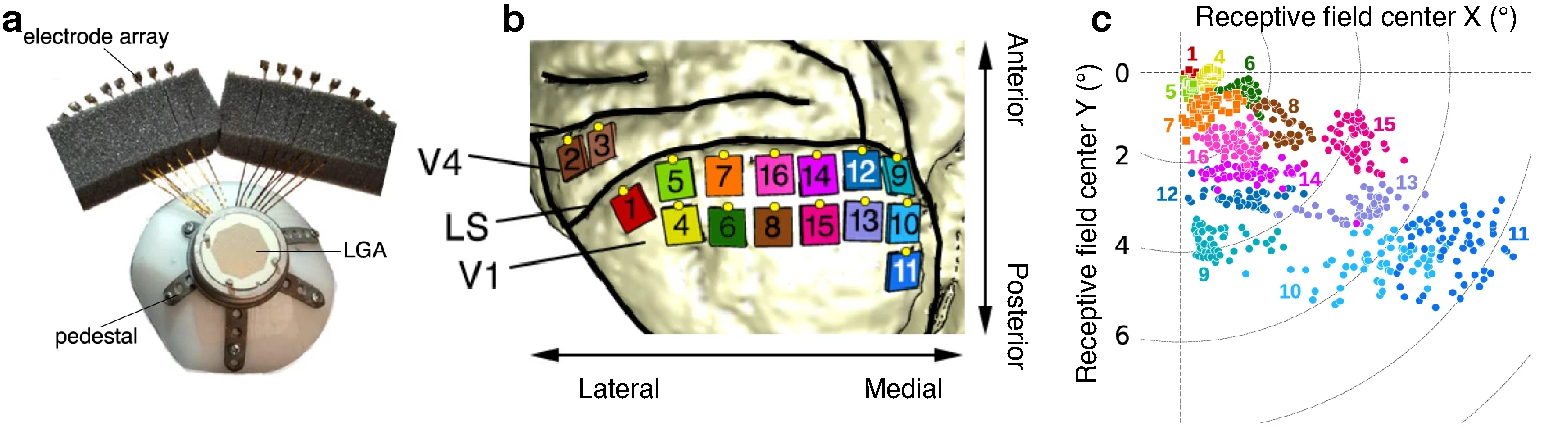
\includegraphics[width=1.\textwidth]{fig/chap5_1024chans.pdf}
\caption[Utah array recording in macaques.]{Typical setup of Utah array recording in macaque visual cortex, similar but not identical to the one used in the present chapter. (a) Example of a macaque implant, consisting of 1024 channels encased in a titanium cranial pedestal. (b) Typical layout of the arrays. Here, "only" 8 arrays, i.e. 512 channels, are implanted in \gls{V1}. (c) Typical eccentricity of the receptive field, as recorded here. Reproduced from~\cite{chen20221024}.}
\label{fig_chap5_1024chans} 
\end{figure} 

\gls{MUA} was recorded in $8$ Utah arrays, consisting of $8x8$ electrodes, hence totaling a number of $512$ electrode sites (Figure~\ref{fig_chap5_1024chans}). Given that the implantation of the chamber was done for another set of experiments, it was necessary to remove certain recording sites that were no longer yielding good signal~\cite{super2005chronic}. A signal-to-noise ratio was measured, based on evoked activity over resting ($300$ ms before evoked) baseline. This ratio was measured as the peak activity subtracted by mean resting activity, and normalized by the standard deviation of that resting activity~\cite{chen20221024}. Channels with a signal-to-noise ratio below $1$ were removed from further analysis, leaving $384$ electrodes. As in chapter 4, the circular variance served as a criterion for exclusion of untuned neurons. A threshold was set at $0.85$, removing untuned electrodes and leaving a final $188$ electrodes for analysis.

We thus aimed to analyze how information transfer between each of the remaining $188$ electrodes is affected by input variance. There are numerous ways ($237$, to be exact~\cite{cliff2023unifying}) to measure pairwise interactions between sets of time-based data, and each method comes with its unique benefits and limitations. Here, we decided to measure covariance, which is one of the simplest and most intuitive methods available, and represents how much two electrodes evolve together. This covariance matrix is similar to the matrix form of variance, but extended to multiple variables, as used in the matrix formulation of predictive processing (Equation~\ref{eq_pc_matrix}). Given a pair of electrodes $X$ and $Y$, the covariance at a single timepoint is: 
\begin{equation}
    \text{Cov}(X, Y) = \frac{\sum_{i=1}^{n} (X_i - \bar{X})(Y_i - \bar{Y})}{n-1}
\end{equation}
where  \( X_i \) and \( Y_i \) are the individual values of the signal in electrodes \( X \) and \( Y \) for a given trial $i$, \( \bar{X} \) and \( \bar{Y} \) are the mean values accross trials, and $n$ is the number of trials (here, $40$).

Not only is covariance straightforward to compute and interpret, but its matrix inverse is also useful, as it is the inverse variance matrix, which is the central focus of this thesis. When dealing with large datasets, like ours with $188$ variables (electrodes) but only $40$ observations (trials), directly inverting the covariance matrix can lead to instability due to the disproportionate ratio of variables to observations. To address this, we employ a technique known as a "shrinkage estimator". This method provides a more reliable estimation of the inverse covariance matrix, making it feasible for inversion. Here, we used the common Ledoit-Wolf estimator, which given a matrix $M$: 
\begin{equation}
    \hat{\Sigma}_{LW} = \alpha \cdot \text{F} + (1 - \alpha) \cdot \text{M}
\end{equation}
where \( \hat{\Sigma}_{LW} \) is the Ledoit-Wolf shrinked matrix, \( \alpha \) controls a shrinkage intensity, \( \text{F} \) is the target matrix (the identity matrix scaled by the average variance) and \( \text{M} \) is our sample covariance matrix. Here, $\alpha$ is automatically chosen to minimize the mean squared error of the reconstruction~\cite{ledoit2004well}~\footnote{A year before the publication of this article, these authors released a related article entitled "Honey, I Shrunk the Sample Covariance Matrix"~\cite{ledoit2003honey}. For some reason, the author of the present manuscript found this amusing enough to be note-worthy, and even considered at one point that it would make an excellent title for this chapter. This was eventually decided against, and regarded as a sign that it might be time to stop working on inverse variance-weighting and graduate.}.
The inverse variance matrix (or precision matrix), is thus $\hat{\Sigma}_{LW}^{-1}$.

A property of covariance matrices, and thus of inverse variance matrices, is their symmetry: the interaction between the electrode $X$ and $Y$ is the same as the interaction between electrode $Y$ and $X$. As a result, the interactions we observe between electrodes in this context are not directional; they only have varying degrees of intensity, or weight. While directional metrics might be useful for uncovering how information is transferred between neurons, potentially exposing interactions that are unique to specific orientations, this is being the scope of the current research.

We visualized these matrices as graphs, which are composed of nodes (representing electrodes) and edges (indicating covariance or inverse variance). This graphical representation makes it easier to comprehend the data, as the matrices in their raw form are not readily interpretable. Additionally, this approach offers a range of mathematical tools to analyze network variations. Here, the graphs are non-directional (because of the covariance or precision symmetry), cyclic (because they form closed interactions loop) and weighted (by the co-variance/inverse variance). 
To manage complexity and minimize noise, we binarized these graphs. This means we disregarded edges below a certain threshold, as a $188^2=35344$ edges-wide graph would be too unstable for analysis. We retained only those edges that ranked above the 75th percentile in weight distribution, a common practice in graph theory analyses~\cite{farahani2019application}, This narrowed the focus on the most significant interactions within the network, at the cost of full network representation.

The specific nature of the graphs we've created here limits the range of questions we can explore regarding their topology. To navigate this, we've selected six key metrics to analyze: clustering, centrality, assortativity, neighboring connectivity, small-worldness, and the Wiener Index~\cite{meunier2010modular,bullmore2012economy}. Mathematical details are provided hereafter, but are not necessary for the comprehension of the results. Rather, an intuitive description is provided with each equation, and a graphical representation is shown in Figure~\ref{fig_chap5_graph_metrics}.

\begin{figure}[h!tbp]
\vspace{0.1cm}
\centering
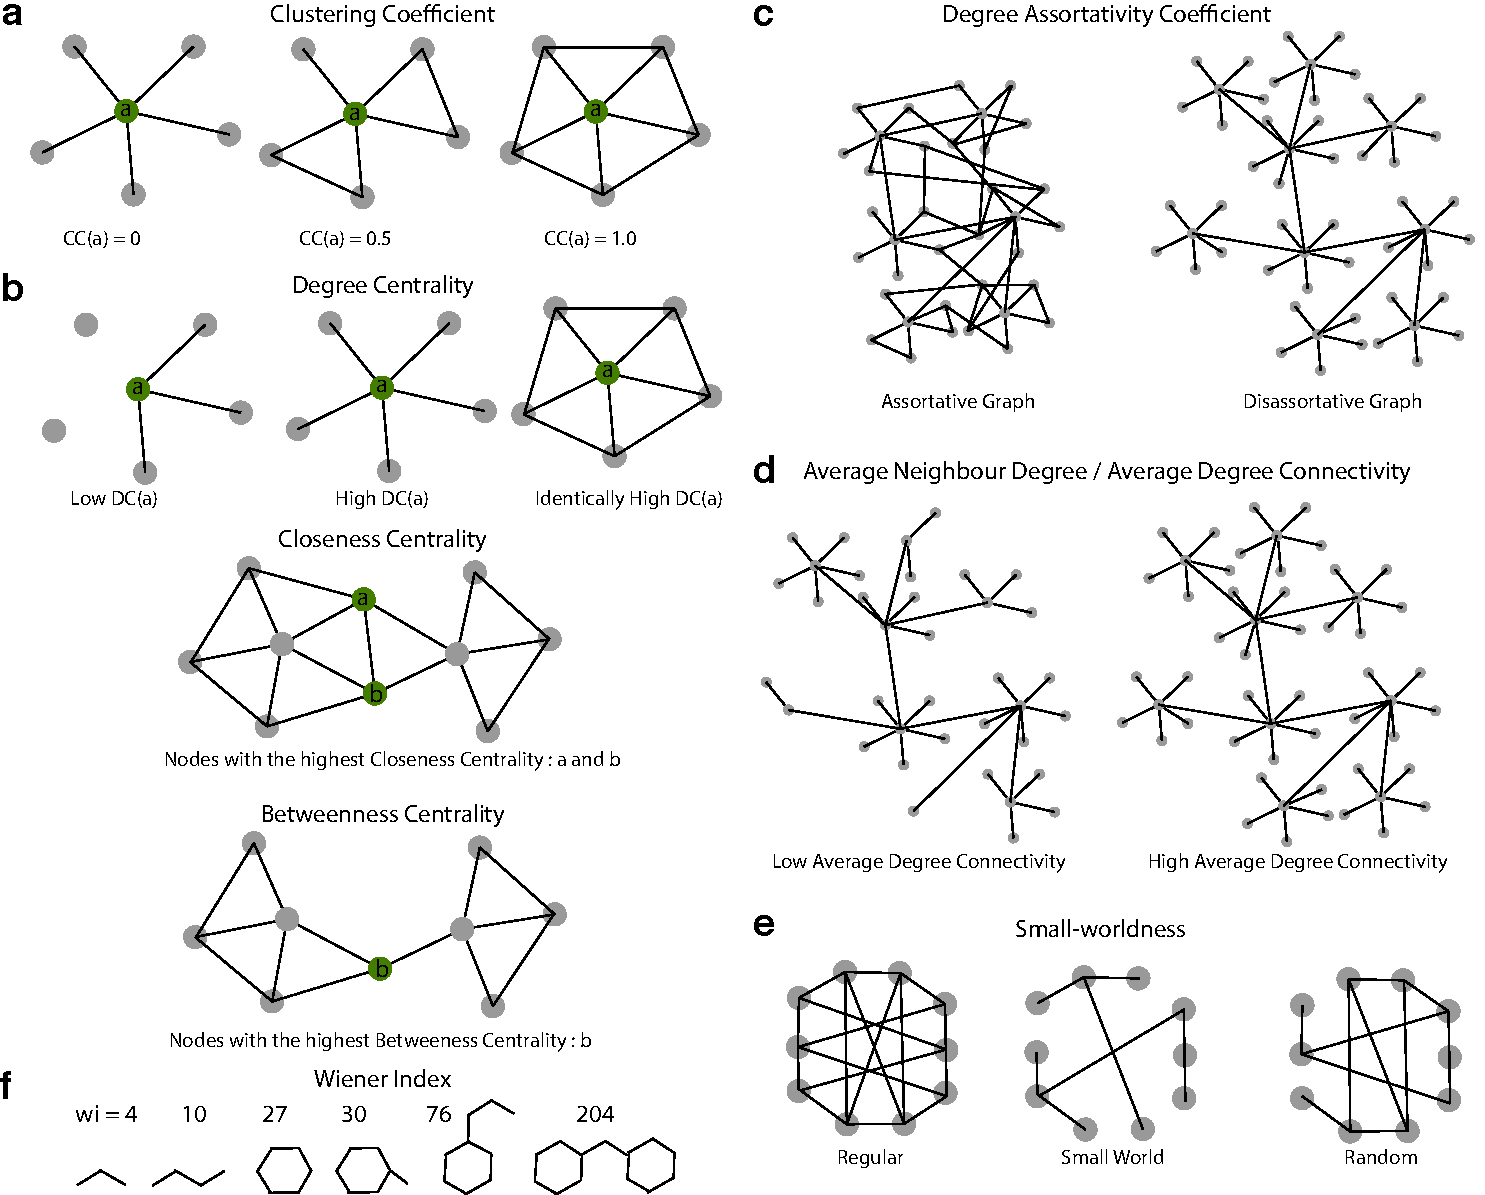
\includegraphics[width=1.\textwidth]{fig/chap5_graph_metrics.pdf}
\caption[Graph metrics.]{Graph metrics, presented in identical order as in the text below. (a) Clustering Coefficient, (b) Centrality metrics, (c) Degree Assortativity Coefficient, (d) Average Connectivity Metrics, (e) Small-worldness index, (f) wiener Index, represented onto common chemical compounds (delocalized electron cycles not shown).}
\label{fig_chap5_graph_metrics} 
\end{figure} 

The first metric used is the clustering coefficient, a measure of the degree to which nodes in a graph tend to cluster together. For example, in the context of a social graph, it helps understand the extent to which friends of a given person are also friends between each other. Here, it can be seen as a direct measure of the global interconnectedness of the neural network being recorded.
The equation for the clustering coefficient \( C_i \) of a node (electrode) \( i \) in a graph is:
\begin{equation}
    C_i = \frac{2T(i)}{k_i(k_i - 1)}
\end{equation}
where \( T(i) \) is the number of triangles through the node \( i \) (i.e., the number of connections that exist among the immediate neighbors of the node \( i \)) and \( k_i \) is the degree of node \( i \) (i.e., the number of edges connected to node \( i \)). \( C_i \) ranges from 0 to 1, with higher values meaning a greater degree of clustering. Here, all node-wise metrics were reported as a distribution of values across multiple input $\theta$, for each $B_\theta$.

A second metric, or rather, class of metric, is the measure of centrality. Multiple sub-metrics are available here, each with their own importance. We measured three, which are:
\begin{itemize}
    \item Degree Centrality: The simplest form of centrality. For a node in a graph, degree centrality is simply the count of how many connections (edges) it has. Nodes with higher degree of centrality are typically more influential or important in a network because they have more connections. Thus, the higher the overall Degree Centrality of a graph is, the more connected the graph is. Following the equation above, it is thus simply measured as $k_i$.
    
    \item Closeness Centrality: This centrality metric focuses on how close a node is to all other nodes in the network. It is defined as the reciprocal of the sum of the shortest path distances from a node to all other nodes in the network. A higher closeness centrality indicates that a node can spread information to all other nodes in the network through less synapses. It is often correlated with the metric above, but not necessarily (see Figure~\ref{fig_chap5_graph_metrics} for example). For a given node \( v \), the closeness centrality \( C_C(v) \) is:
    \begin{equation}
        C_C(v) = \frac{1}{\sum_{u \neq v} d(v, u)}
    \end{equation}
    where \( d(v, u) \) is the shortest-path distance between nodes \( v \) and \( u \), and the sum is taken over all nodes \( u \) in the graph except \( v \) itself.
    
    \item Betweenness Centrality: This centrality metric quantifies the number of times a node acts as a bridge along the shortest path between two other nodes. It captures the degree to which a node lies on paths between others, indicating its potential for control over information flow in the network. Nodes with higher betweenness centrality can have significant influence within a network, by virtue of their ability to gate message passing between other nodes. For a given node \( v \), the betweenness centrality \( C_B(v) \) is calculated as:
    \begin{equation}
        C_B(v) = \sum_{s \neq v \neq t} \frac{\sigma_{st}(v)}{\sigma_{st}}
    \end{equation}
    where \( \sigma_{st} \) is the total number of shortest paths from node \( s \) to node \( t \), \( \sigma_{st}(v) \) is the number of those paths that pass through \( v \). The sum is computed over all pairs of nodes \( s \) and \( t \) in the graph, where \( s \neq t \neq v \).
\end{itemize}

A third metric is the Degree Assortativity Coefficient. It measures the tendency of nodes to connect to other nodes which have similar degrees. In other terms, it reflects whether high-degree nodes (nodes with many connections) tend to be connected to other high-degree nodes, and similarly for low-degree nodes. The Degree Assortativity Coefficient \( r \) can be calculated using the Pearson correlation coefficient for degree-degree pairs across all edges in the network. The formula is as follows:
\begin{equation}
    r = \frac{\sum_{jk} jk (e_{jk} - q_j q_k)}{\sigma_q^2}
\end{equation}
where \( e_{jk} \) is the proportion of edges in the network that connect a node of degree \( j \) to a node of degree \( k \), \( q_j \) is the proportion of ends of edges that are attached to nodes of degree \( j \) (also known as the "normalized degree distribution") and \( \sigma_q^2 \) is the variance of the distribution \( q \). The assortativity coefficient \( r \) ranges from -1 to 1. A value of 1 indicates perfect assortative mixing patterns, 0 indicates non-assortative mixing, and -1 indicates perfect disassortative mixing. Understanding the degree assortativity of a network is essential in analyzing the robustness and the dynamics of information or disease spread within the network. Thus, if high-degree nodes tend to connect with low-degree nodes, the network exhibits negative degree assortativity, as shown here. 

Fourth are degree metrics, namely, the Average Neighbor Degree and the Average Degree Connectivity. 
The Average Neighbor Degree is a measure for each node in a network, that is the average degree of its neighboring nodes. This measure is useful for understanding the tendency of nodes to connect to others that are similarly well-connected or not; much like the Degree Assortativity Coefficient. For instance, in a network with high degree correlation (assortativity), high-degree nodes tend to be connected to other high-degree nodes. For a node \( v \) with degree \( k \), the Average Neighbor Degree \( \text{AND}(v) \) is given by:
\begin{equation}
    \text{AND}(v) = \frac{1}{k} \sum_{u \in N(v)} \deg(u) 
\end{equation}
where \( N(v) \) denotes the set of neighbors of \( v \), and \( \deg(u) \) is the degree of a neighbor \( u \). 
The Average Degree Connectivity, on the other hand, is a network wide metric that measures the average degree of the neighbors of nodes with a given degree. As such, it is often correlated with the $\text{AND}$. The Average Degree Connectivity for nodes of degree \( k \) in a network, denoted as \( \text{ADC}(k) \), is defined as:
\begin{equation}
    \text{ADC}(k) = \frac{1}{N_k} \sum_{v: \deg(v) = k} \text{AND}(v)
\end{equation}
where \( N_k \) is the number of nodes with degree \( k \) in the network. Their interpretation, similar to the Assortativity Coefficient, gives insight into whether the network is assortative or disassortative (Figure~\ref{fig_chap5_graph_metrics}).

A fifth metric is the degree of small-worldness, which quantifies a network in which clustering coefficient is high, while maintaining short average path length. In neural networks, this results from the balance between minimizing the resource cost and maximizing the flow of information among the network components. In brain-wide networks, the metabolic cost between neighboring neurons is much lower than that of distant neurons, and thus the brain behaves a small-world network~\cite{liao2017small} to increase efficiency, as described in the introduction of this manuscript~\cite{barlow1961possible}.
A direct measure of small-worldness compares the current graph with a random network~\cite{watts1998collective}. This measure of small-worldness quantifies the balance between local clustering and global reach in a network. Specifically, small-world networks have significantly higher clustering than random graphs but similar average path lengths. Thus, the small-worldness \( S \) of a network can be quantified as follows:
\begin{equation}
    S = \frac{C / C_{random}}{L / L_{random}}
\end{equation}
where \( C \) is the average clustering coefficient of the network, \( L \) is the average shortest path length of the network, \( C_{random} \) and \( L_{random} \) are the average clustering coefficient and average shortest path length, respectively, of an equivalent random graph. Typically, a network is considered to exhibit small-world properties if \( S > 1 \), indicating that it has higher clustering than a random graph while maintaining a comparable average shortest path length. 

Finally, a sixth metric is the Wiener Index, one of the oldest topological indices~\cite{diudea1998wiener} that is used primarily in chemical graph theory (see Figure~\ref{fig_chap5_graph_metrics}). It is a measure of the compactness of a network and is closely related to the small-worldness and efficiency of the network.
 The Wiener Index \( W \) of a network is defined as:
 \begin{equation}
     W = \sum_{\{i,j\} \subseteq G} d(i, j)
 \end{equation}
which is the sum of the shortest path lengths between all pairs of nodes in the graph. In this context, \( G \) is the set of nodes in the network, and \( d(i, j) \) represents the shortest path between nodes \( i \) and \( j \).



\section{Results: Modulations of Connectivity Patterns by Orientation Variance}
Before diving into graph metrics, let us first assess direct \gls{V1}-based metrics. Namely, we will first observe whether the variance-tuning curves shown in chapter 4 are also present in primate \gls{V1}. In this part of our study, the reliance on \gls{MUA}, rather than single-neuron activity,  means we lose the granularity of precise spike timing. There are however notable parallels in how both \gls{MUA} and single neuron activities in terms of orientation tuning~\cite{lange2023weak}. 

This holds true here, as the variance-tuning functions reveal similar patterns of activity modulation across neurons as shown in chapter 4. Despite the shift in scale from single neurons to \gls{V1}, we observe a comparable distribution of heterogeneous modulations in neuronal activity, as shown in Figure~\ref{fig_chap5_nkr}. This validates the consistency of our findings across different levels of neural activity and species. This, in turns, allows us to extrapolate (with caution) some similarities between the precise single-neuron mechanism of chapter 4 and the graph metrics of this chapter.

\begin{figure}[h!tbp]
\vspace{0.1cm}
\centering
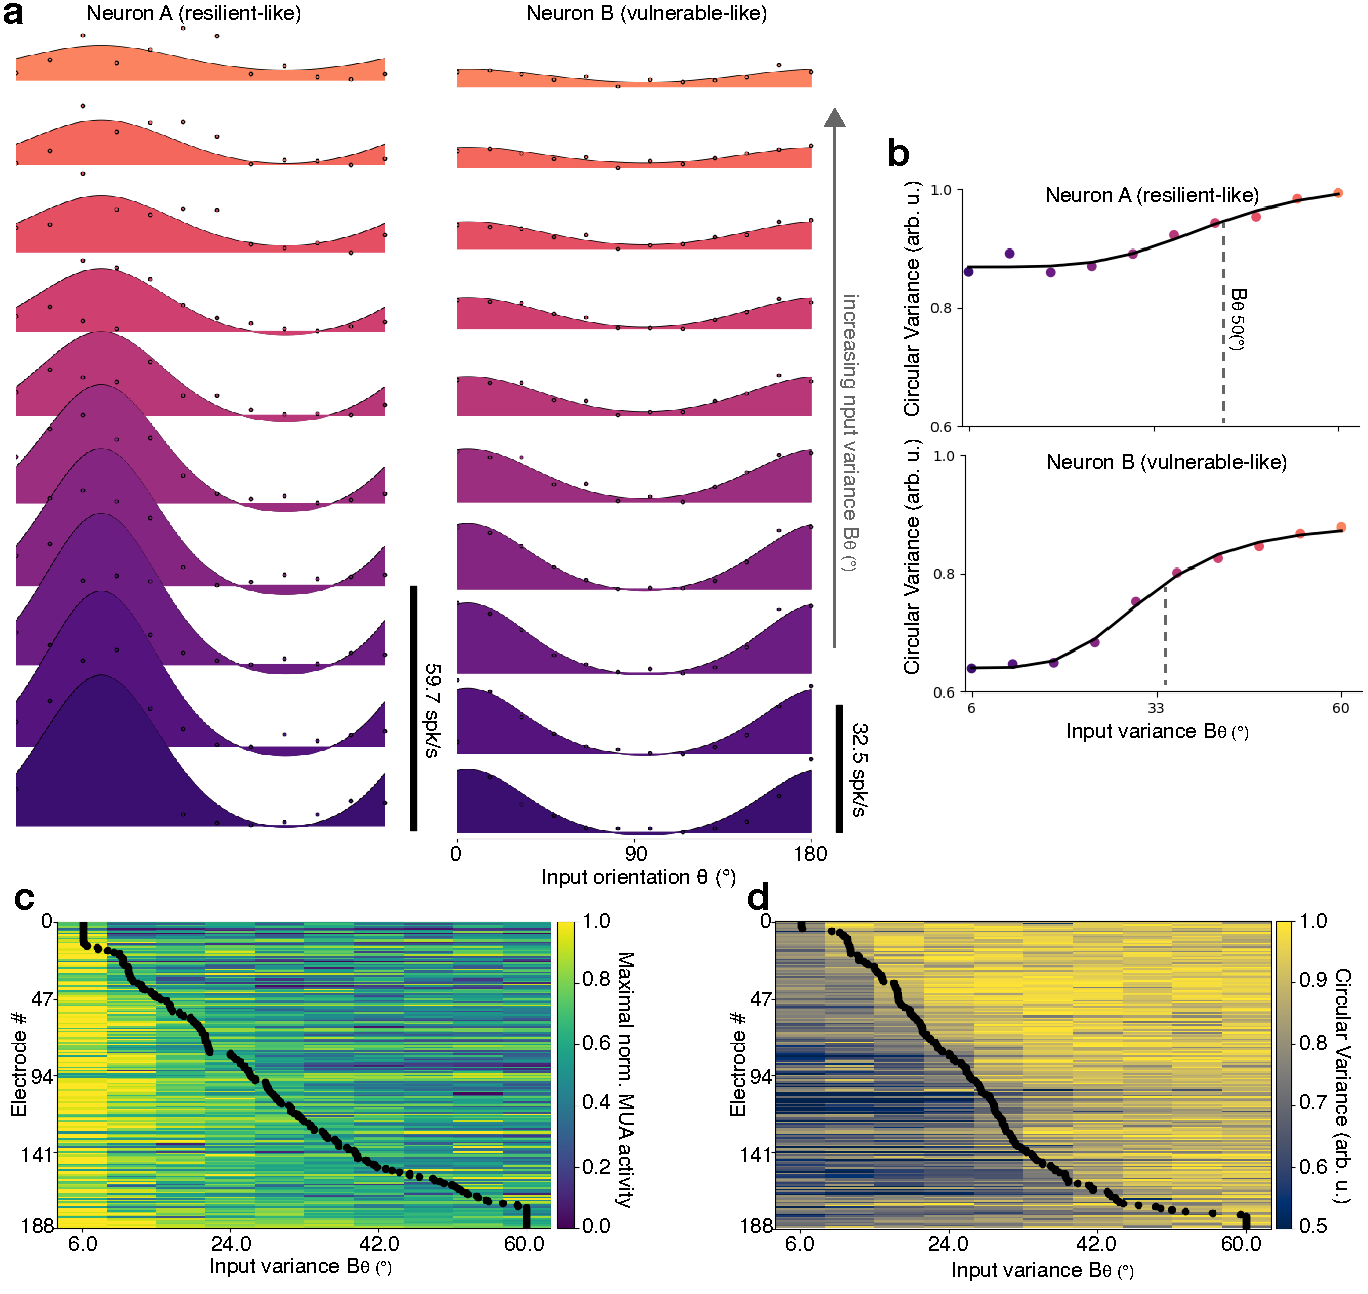
\includegraphics[width=1.\textwidth]{fig/chap5_nkr.pdf}
\caption[Variance tuning functions in primate V1.]{Variance tuning functions in primate \gls{V1}. (a) Modulation of tuning curve for two example \gls{MUA}, reminiscent of resilient/vulnerable neurons described in chapter 4. (b) Variance-tuning functions of these two examples \gls{MUA}, fitted with a Naka-Rushton function (black line). (c) Population map of variance-tuning functions, with dots representing $B_{\theta50}$, the changepoint of the function (see chapter 4). (d) Population map of variance-tuning functions, as with (c).}
\label{fig_chap5_nkr} 
\end{figure} 

While timing modulations are present (data not shown), in practice, these were on the order of tens of milliseconds in single neurons (i.e., about one $\tau$), and thus, it would be hard to extrapolate these in \gls{MUA} due to smoothing across multiple neurons. Given these constraints, our analysis at the single-electrode level is largely limited to tuning metrics. Hence, we turn our focus to mesoscale measurements, which offer a broader view of neural activity while still providing valuable insights. 
An example of such a mesoscale measurement is neural decoding, as we explored in chapter 4. Decoding would have been a particularly interesting approach in this context, especially since the activity is recorded in physical simultaneity, as opposed to virtually concatenated in chapter 4. Given similiarities in tuning, we might hypothesize that the decoding results in primate \gls{V1} would mirror those found in cat. This assumption is based on the consistent tuning characteristics observed across different animal models, suggesting a fundamental similarity in how \gls{V1} processes visual information.

However, here, we tried to branch away from simply reproducing chapter 4 results, and opted to investigate the interactions between neurons, as opposed to decoding an emergent neural code. As detailed in the methods section, to explore this, we utilized covariance matrices and their inverses, the inverse variance matrices, as our primary analytical tools.
For the $188$ electrodes, such matrices are shown in Figure~\ref{fig_chap5_matrices}. These represent the interactions between neurons, and characterize the variation of recurrent message passing between neurons. Here, there are measured for a single input $\theta$, which was chosen as the one with most \gls{MUA} tuned onto. We reasoned that this would be the orientation for which the representation would be the most accurate, but we will then average metrics across orientations in later sections.

\begin{figure}[h!tbp]
\vspace{0.1cm}
\centering
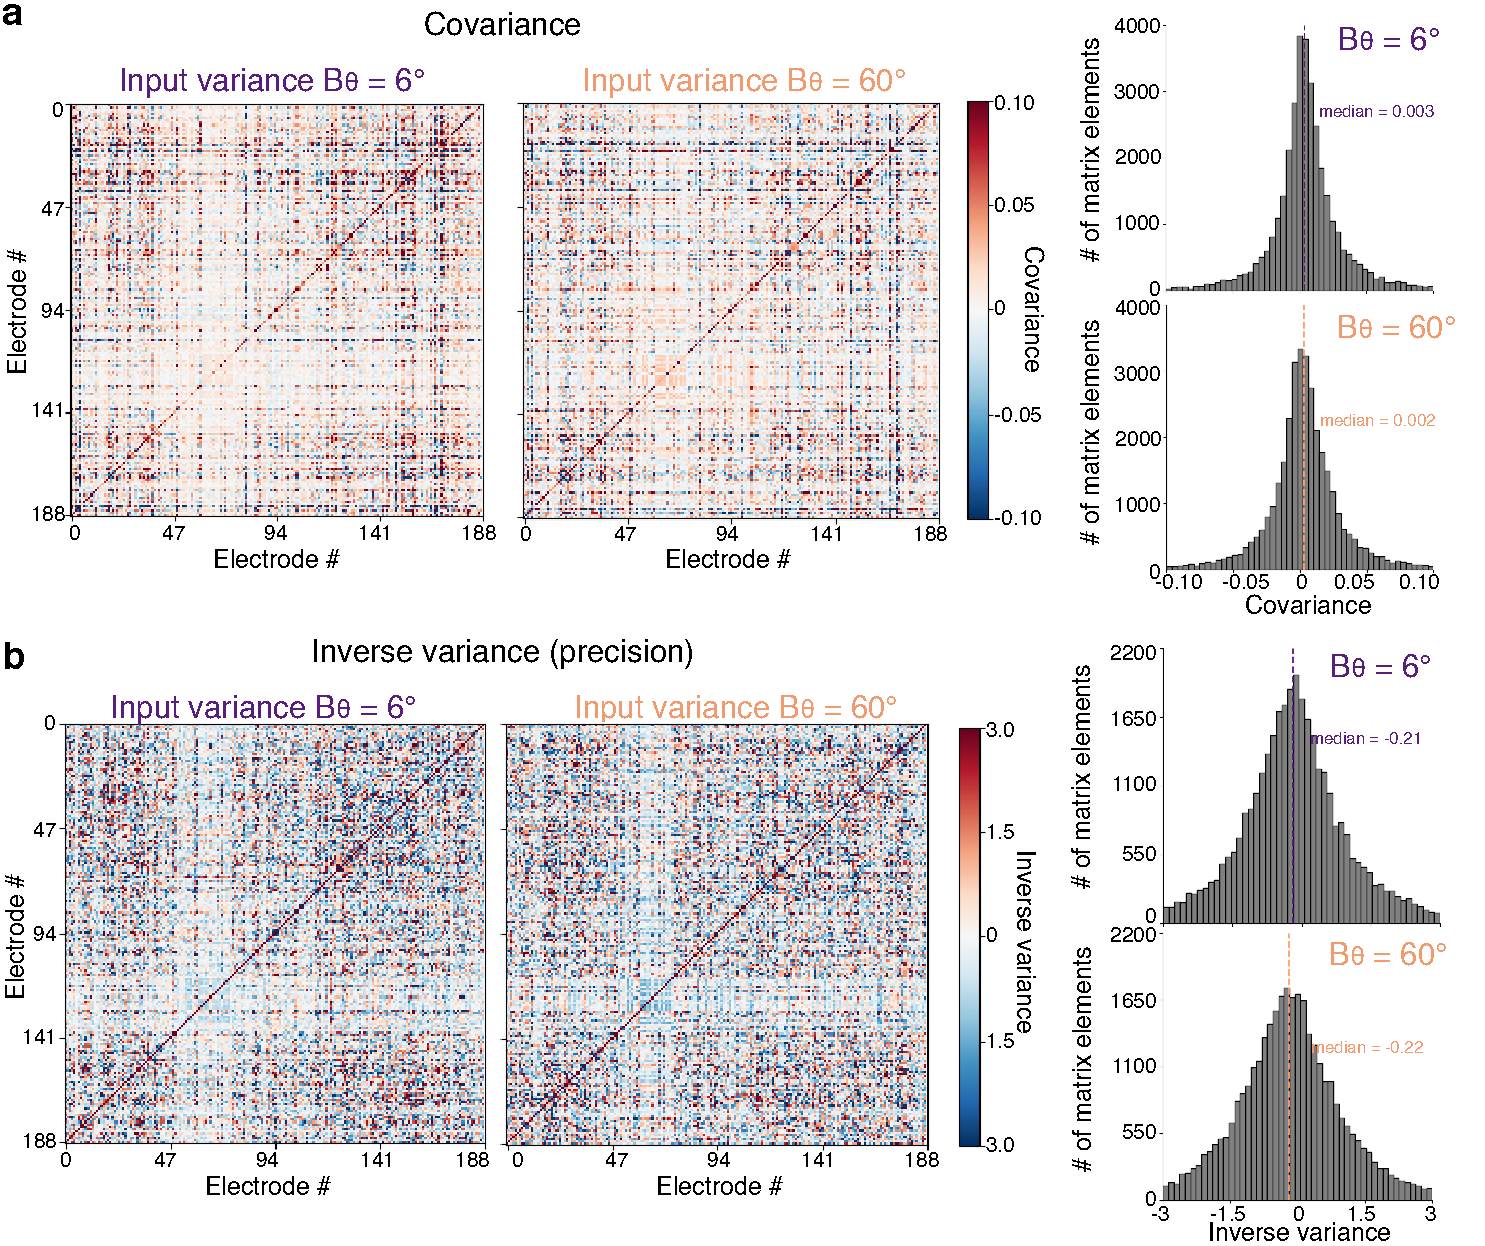
\includegraphics[width=1.\textwidth]{fig/chap5_matrices.pdf}
\caption[Covariance matrices in primate V1.]{Inverse variance-weighting in primate \gls{V1}. (a) Covariance matrices for lowest and highest variances, for a single orientation. The order of the elements, from $0$ to $188$, follows the preferred orientation at each electrode. Distribution of the covariances values with median value is shown in the right. (b) Same as (a), but for inverse variance (precision) matrices. }
\label{fig_chap5_matrices} 
\end{figure} 

Interpreting connectivity differences solely from the matrices can be challenging, and one often sees what they wish to be true. Even employing ratios or advanced metrics like the Laplacian or matrix-norm doesn't significantly enhance our understanding of these interactions. To mitigate this, we later broaden our approach to average across different orientations, aiming to capture a more comprehensive view of neuronal interactions across the visual spectrum. This expanded analysis is part of our ongoing effort to better understand the intricate web of connections and influences within neural networks.

Thus, it is better to embed these matrices into graphs, which offers better representations and better metrics. These graphs can be plotted onto a tuning ring, where each node's preferred orientation corresponds to a specific position on the circle. This is a neurobiological realization of the computational "ring" model we presented in chapter 4. By positioning neurons according to their orientation preferences, we create a visual map that reflects the inherent structure of neural preferences and interactions in the visual cortex. This is shown in Figure~\ref{fig_chap5_circ_graphs}, which shows a clear variation on the condition of interactions.

\begin{figure}[h!tbp]
\vspace{0.1cm}
\centering
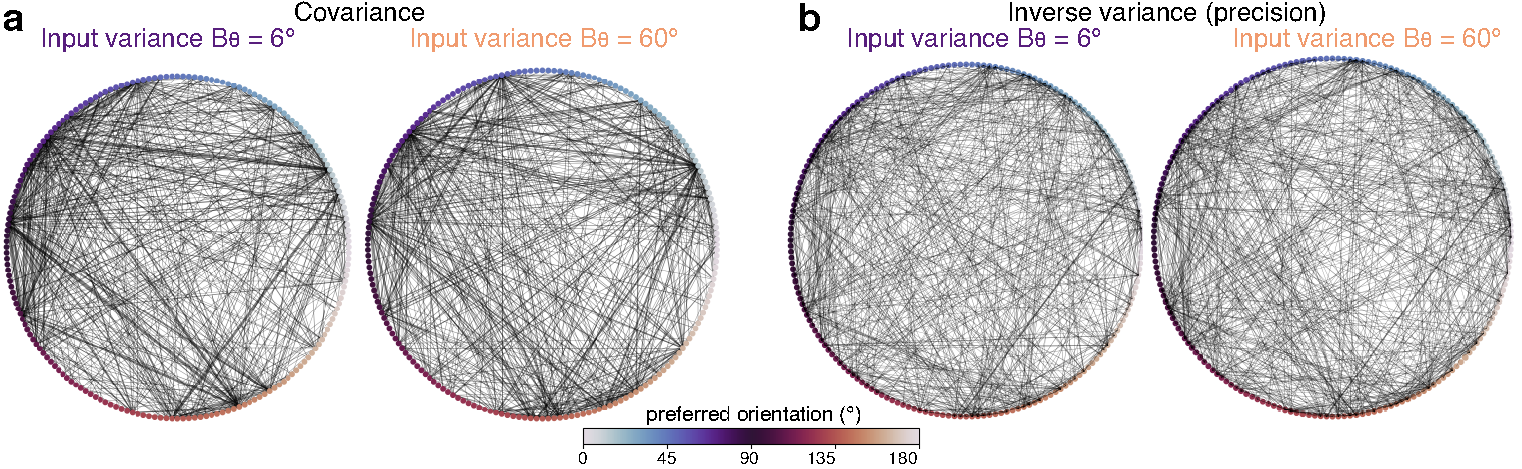
\includegraphics[width=1.\textwidth]{fig/chap5_circ_graphs.pdf}
\caption[Circular graphs of inverse variance.]{Circular graphs of inverse variance-weighting in primate \gls{V1}. (a) Graphs of covariance, with units sorted by their preferred orientations, for lowest and highest variances. (b) Same as (a), but for inverse variance.}
\label{fig_chap5_circ_graphs} 
\end{figure} 

This translates into an immediate, non-scientific conclusion: increasing the variability of input tends to complexify the graph's appearance. There is little to interpret with these representations, as the graph used here are fully connected (due to being based on covariance matrices).
How does this translate into pratical interactions? A more effective method for visualizing these graphs is through a force-directed algorithm, specifically the Fruchterman-Reingold force-directed algorithm, often referred to as a spring layout~\cite{fruchterman1991graph}. This attempts to maintain a certain distance between each node, essentially pushing them apart, but holding them together through their interactions. For instance, positive inverse variance-weighting draws the nodes closer, whereas negative weighting drives them even further apart. This represents the graph in a manner where all the connections (edges) are relatively equal in length and overlap as little as possible, creating a graph that is more straightforward to comprehend. This is shown in Figure~\ref{fig_chap5_force_graphs}.

\begin{figure}[h!tbp]
\vspace{0.1cm}
\centering
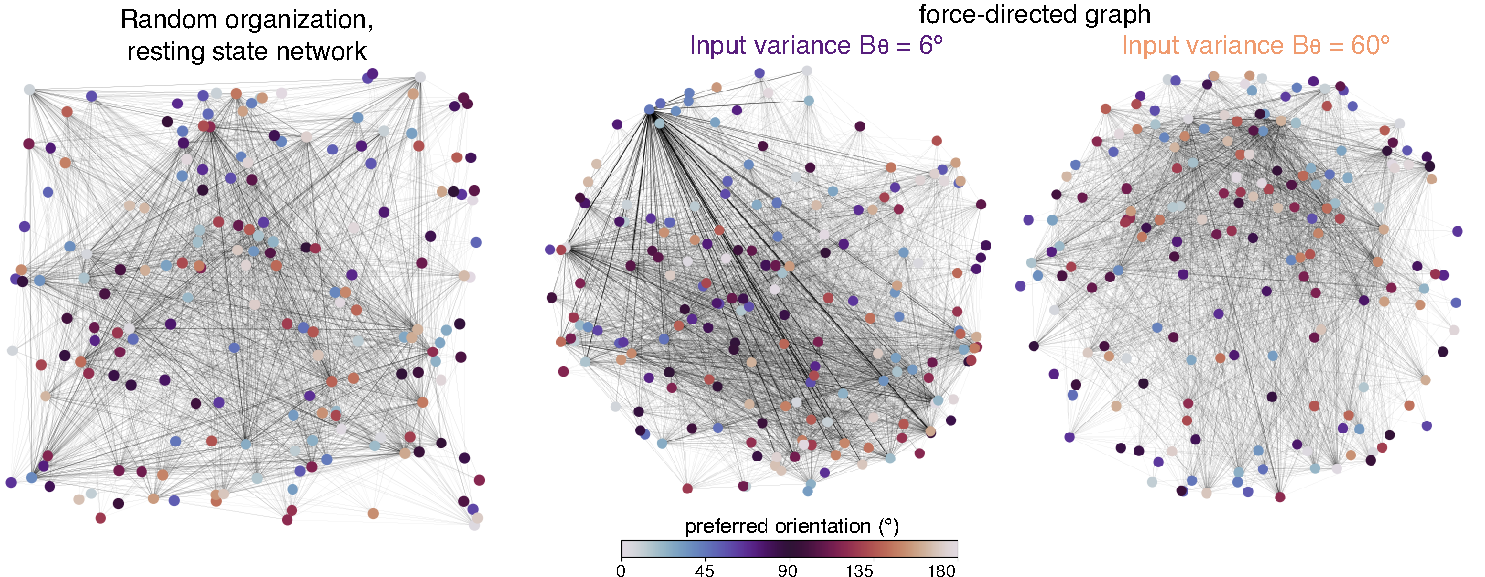
\includegraphics[width=1.\textwidth]{fig/chap5_force_graphs.pdf}
\caption[Force-directed graphs of inverse variance.]{Force-directed graphs of inverse variance-weighting in primate \gls{V1}, initialized from random positions (left), for lowest (middle) and highest variance (right).}
\label{fig_chap5_force_graphs} 
\end{figure} 

This is now steering us towards a clearer interpretation of the graph's dynamics. Through these representations, it becomes evident that with maximum input variance, the network's structure transitions from a dense, small-world configuration (concept introduced in Figure~\ref{fig_chap5_graph_metrics}) to a more dispersed, globally distributed network. This observation aligns with the concepts introduced in chapter 4, namely the idea that computations within the network become more iterative and distributed when dealing with high variance, in contrast to being more concentrated and feedforward-based for inputs with low variance. 

To properly quantify this phenomenon, we will now turn to the metrics that have been described in the methods section above (Figure~\ref{fig_chap5_quantification_graphs}). In the order in which they have shown in Figure~\ref{fig_chap5_graph_metrics}, these metrics paint a converging picture:
\begin{itemize}
    \item Clustering Coefficient increases as a function of input variance (Mann-Whitney U test between $B_\theta = 0$° and $60$° : $U=0.0, p<0.0001$. Linear regression : $y = 0.004x+0.68$, $p = 0.01$).
    Intuitively, this means that the neural activity in \gls{V1} is becoming more interconnected, as opposed to separated into uncorrelated sub-networks. This implies a shift from isolated processing to more integrated, recurrent neural activity, where neurons are not just operating independently, but are increasingly interlinked.
    
    \item Degree Centrality ($U=1968.5, p<0.0001$. lin. reg. : $y = 0.006x+0.65$, $p = 0.005$) and Closeness Centrality ($U=1994.0, p<0.0001$. lin. reg. : $y = 0.003x+0.74$, $p = 0.006$) increase as a function of input variance.
    This gives a similar interpretation as with the Clustering Coefficient, that of a network whose units are processing information in a more distributed fashion. Betweenness Centrality, however, is decreasing with input variance, ($U=19555.0, p<0.0001$. lin. reg. : $y = -0.00003x+0.001$, $p = 0.005$), suggesting that fewer nodes are acting as critical bridges within the network. This could mean that the network is becoming less reliant on given neural pathways, and distributes its processing load more evenly across the network.
    
    \item Degree Assortativity Coefficient is negative for all input variance, but still increases with input variance (lin. reg. : $y = -0.005x-0.05$, $p = 0.0002$).
    This means that a dissasortative neural network is progressively reorganizing into a less-tightly organized assortative neural network. However, as this coefficient absolute value's does increase with variance, it indicates a shift towards a network where nodes are more likely to connect with similar nodes. This transition suggests a move from a more hierarchical or specialized network to a more homogenized one.
    
    \item Average Neighbour Degree is increasing with input variance ($U=0.0, p<0.0001$. lin. reg. : $y = 1.05x+124$, $p = 0.006$). This implies that that neurons are not only increasing their connections but are also tending to connect with other neurons that are similarly highly connected, hinting at a more uniformly interconnected network, where all neurons are part of equally significant ensembles of interactions.
    
    \item Small-worldness is decreasing with variance (lin. reg. : $y = -0.004x+1.06$, $p = 0.001$). This marks a departure from the dominant default-mode of connectivity in neural networks~\cite{meunier2010modular}, and as with Average Neighbour and Average Degree Connectivity, \gls{V1} is becoming less tightly organized and distributed.
    
    \item Wiener Index is decreasing with variance (lin. reg. : $y = -119x+23820.5$, $p = 0.004$). A decrease in this index is intriguing, as it suggests that the overall path lengths within the network are reducing. This could mean that despite the increase in distributed processing, the network is somehow becoming more efficient in terms of signal transmission distances, which could be due to the reorganization of connections in the network. One implication of this is that the seeming disorganization of the network is not so much a disorganization as it is a planned reorganization, into an equally efficient but topologically different neural network.
\end{itemize}
Overall, these findings are very exciting, as they all converge towards a similar observation: with increased input variance, \gls{V1} is actively being reorganized from a tightly segregated topology into a delocalized, recurrent processing neural network. How these metrics evolve through time could also align with the idea of dynamical processing of orientation variance, as exposed in chapter 4, and form a promising avenue of research.

\begin{figure}[h!tbp]
\vspace{0.1cm}
\centering
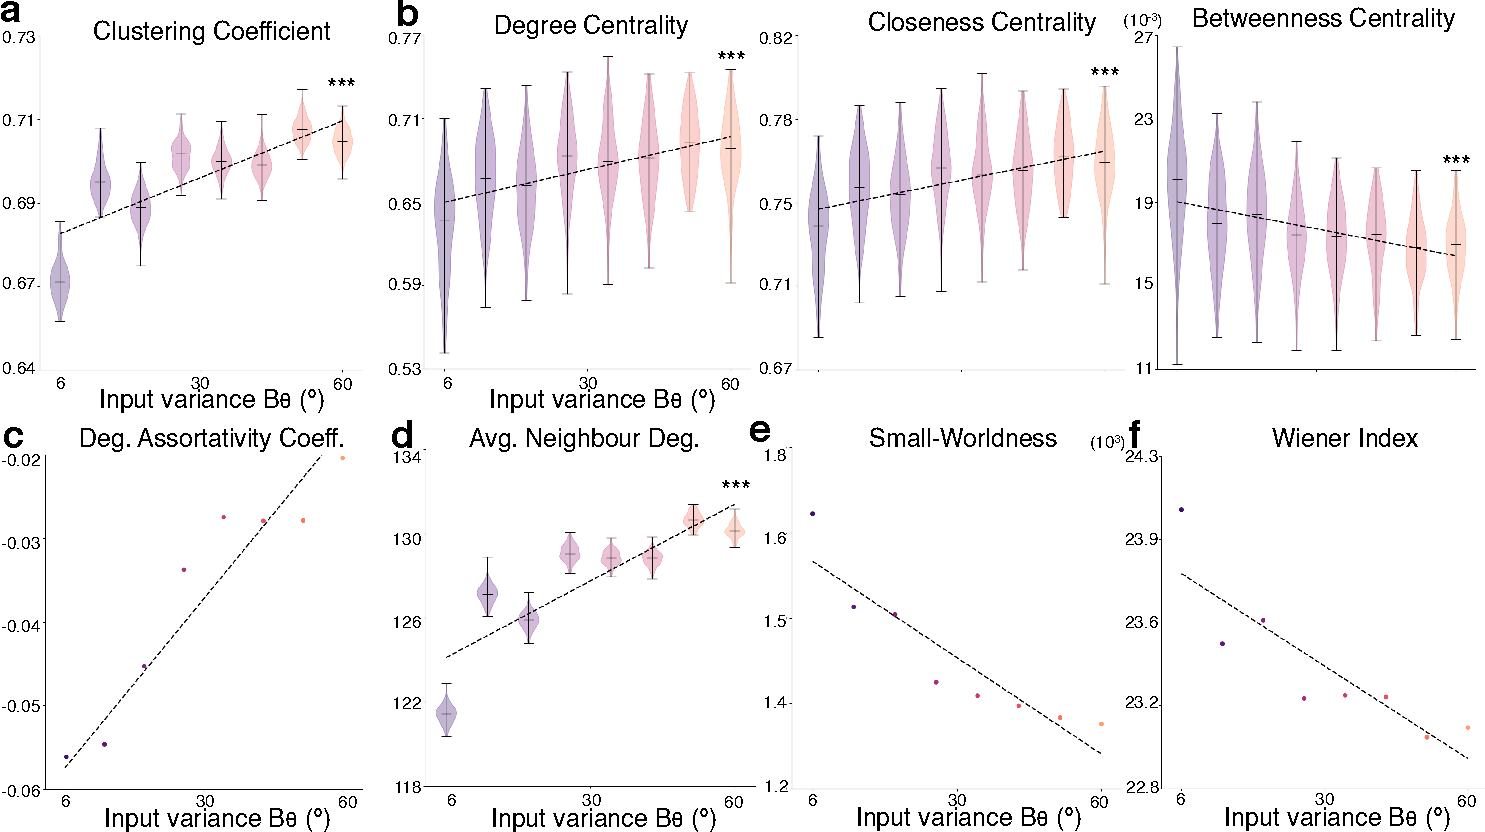
\includegraphics[width=1.\textwidth]{fig/chap5_quantification_graphs.pdf}
\caption[Quantification of graphs.]{Quantification of graphs. (a) Clustering Coefficient, showed as a violinplot with 5th, 95th quartiles and median values. Linear regression is shown as a dashed black line. Significance of the difference between $B_\theta=0$° and $60$° is indicated above the last boxplot (Mann-Whitney U test, $***;p<0.001$, $**;p<0.01$). (b) Centrality metrics. (c) Degree Assortativity Coefficent. (d) Average Neighbour Degree. (e) Small-Worldness. (f) Wiener Index.}
\label{fig_chap5_quantification_graphs} 
\end{figure} 

%These findings also extend the narrative established in chapter 4, aligning with an idea of dynamical processing of orientation variance observed in \gls{V1}.  Just as chapter 4 demonstrated that increased input variance necessitated extended processing time in \gls{V1}, the metrics here observed also show a temporal component. This suggests that the shift towards a decentralized network configuration is not a static alteration, but a dynamic property of the neural network, which could have been observed through the decoding process in chapter 4. TODO MORE HERE

%\begin{figure}[h!tbp]
%\vspace{0.1cm}
%\centering
%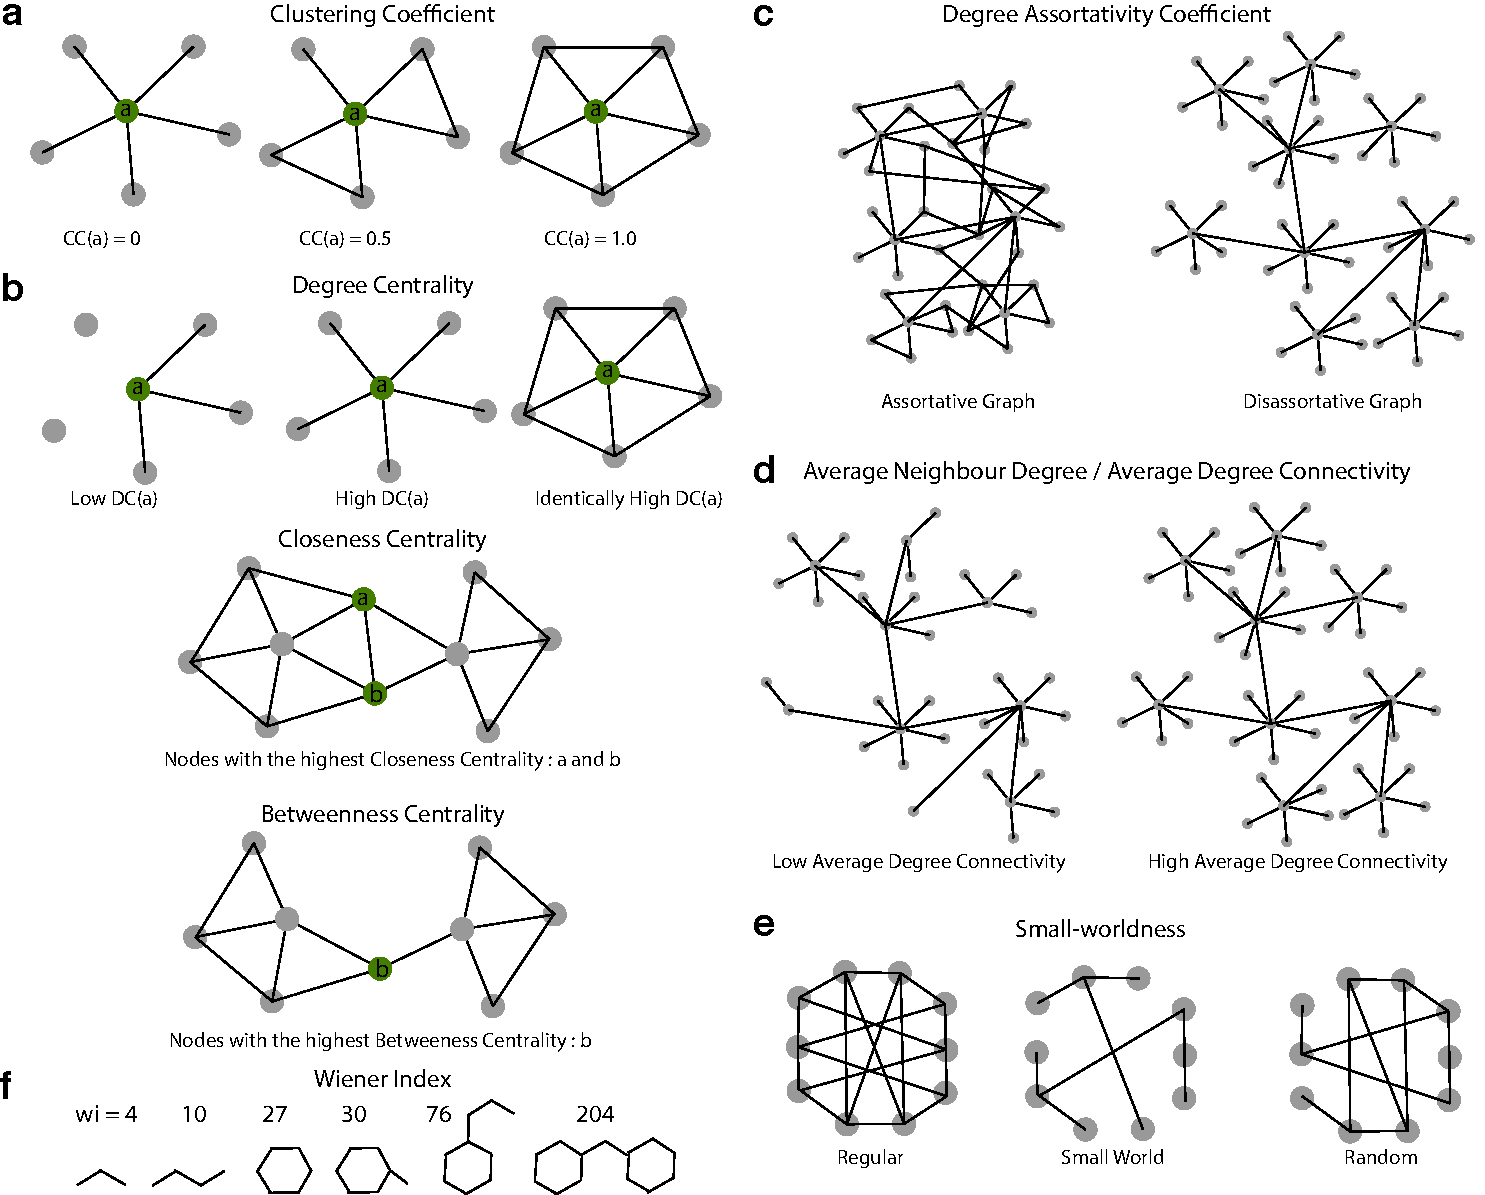
\includegraphics[width=1.\textwidth]{fig/chap5_dynamic_graphs.pdf}
%\caption[Dynamic modulation of graph through time.]{Dynamic modulation of graph through time. (a) }
%\label{fig_chap5_dynamic_graphs} 
%\end{figure} 



\section{Conclusion: A Predictive Coding Perspective}
Graph-based approaches to neuroscience often describes the brain as a small-world network~\cite{liao2017small}, which is a general principle of any system that balances efficiency and minimization of operating cost~\cite{sterling2015principles}. In the context of our manuscript, this means a series of networks that function in tandem, and are coordinated by broader neural interactions. Although the leap is theoretical, these can also be likened to a 'canonical microcircuit' model, where the brain processes sensory information (like orientation) and puts collaboration between adjacent circuits into play to form a comprehensive and integrated model of the environment.

Our research, particularly in Chapter 4, delved into the functional organization within a single cortical area, highlighting how single neurons and populations adapts to different variance in sensory input. We theorized an increase in recurrent neural activity in response to higher input variances.  Here, in awake vigil macaques, we show that is experimentally the case, using a graph theory approach that shows decentralization of the neural network as a function of the sensory input's variance. This aligns with our initial theory that the brain's segregated and linear processes evolve into more interconnected, decentralized operations involving multiple neurons, when faced with complex stimulus. This also implies that experiments based on stimulating \gls{V1} with drifting gratings are missing a crucial key component of the brain, that is, its network capacity to re-organize in face of sensory variance to adjust to an uncertain environment. 

The implications of these findings for predictive coding are significant. Let us now focus on the notion of variance, rather than inverse variance, as this will make more intuitive sense based on a Motion Clouds definition. If input variance increases in the visual input, patterns of activity across multiple orientation-tuned units in \gls{V1} also increase in variance (as also shown in chapter 4). This decentralization of the message passing between neuron implies that the distribution of neural activity, in orientation space, is a function of the distribution of input orientation.
As posited by predictive coding, lower-level (inverse) variance distributions in sensory areas are essential for learning the statistical variance in the environment. Essentially, the brain uses these lower-level distributions to fine-tune its predictions about the inherent variance in both the environment, but also in the sensors used to sample said environment. 

To validate this notion, one could imagine showing repeated high variance input to a macaque, and see how these response changes from a \gls{V1} that is used to process heterogeneous variance. One could then expect systematically broader patterns of activity in \gls{V1}.  Another way to explore these limits is to implement them into a predictive coding model, and see how this model behaves in the face of changing input variance. With the theoretical and mathematical framework already in place in the thesis' introduction, it would be rather straightforward to develop a neural network that implements predictive processing. This network could then be tasked with a simple machine learning classification task, for instance, solving the Modified National Institute of Standards and Technology database, a list of handwritten digits between 0 and 9. This task is trivial, and often the first one to be done on a newly developed neural network. Following this tradition, one could embed these digits into Motion Clouds, thereby manipulating the orientation distributions of these inputs and see whether similarities in the learned inverse variance matrix follow those observed in macaque \gls{V1}.

%As a reminder from $100$ pages ago, the general matrix form equation (i.e., Equation~\ref{eq_pc_matrix}) of predictive coding is:
%\begin{equation}
%    \begin{aligned}
%        \dot{\bar{\varepsilon}}_p &= \bar{\phi} - \bar{v}_p - \mathbf{\Sigma_p}\bar{\varepsilon}_p \\
%        \dot{\bar{\varepsilon}}_u &= \bar{u} - g(\bar{\phi}) - \mathbf{\Sigma_u}\bar{\varepsilon}_u \\
%        \frac{\delta F}{\delta \bar{v_p}} &= \bar{\epsilon}_p \\
%        \frac{\delta F}{\delta \boldsymbol{\Sigma_p}} &= \frac{1}{2}(\bar{\epsilon}_p\bar{\epsilon}_p^T - \boldsymbol{\Sigma_p^{-1}}) \\
%        \frac{\delta F}{\delta \boldsymbol{\Sigma_u}} &= \frac{1}{2}(\bar{\epsilon}_u\bar{\epsilon}_u^T - \boldsymbol{\Sigma_u^{-1}})
%    \end{aligned}
%\end{equation}
%Using Python and PyTorch, a code implementation of these equations is rather straightforward, and can be easily turned into a classification neural network (for details, see also~\cite{millidge2020relaxing}). This network can then be tasked with a simple machine learning classification task, for instance, solving the Modified National Institute of Standards and Technology database, a list of handwritten digits between 0 and 9. This task is trivial, and often the first one to be done on a newly developed neural network. Following this tradition, we will here embed these digits into Motion Clouds, thereby manipulating the orientation distributions of these inputs (Figure~\ref{fig_chap5_mnist}).

%\begin{figure}[h!tbp]
%\vspace{0.1cm}
%\centering
%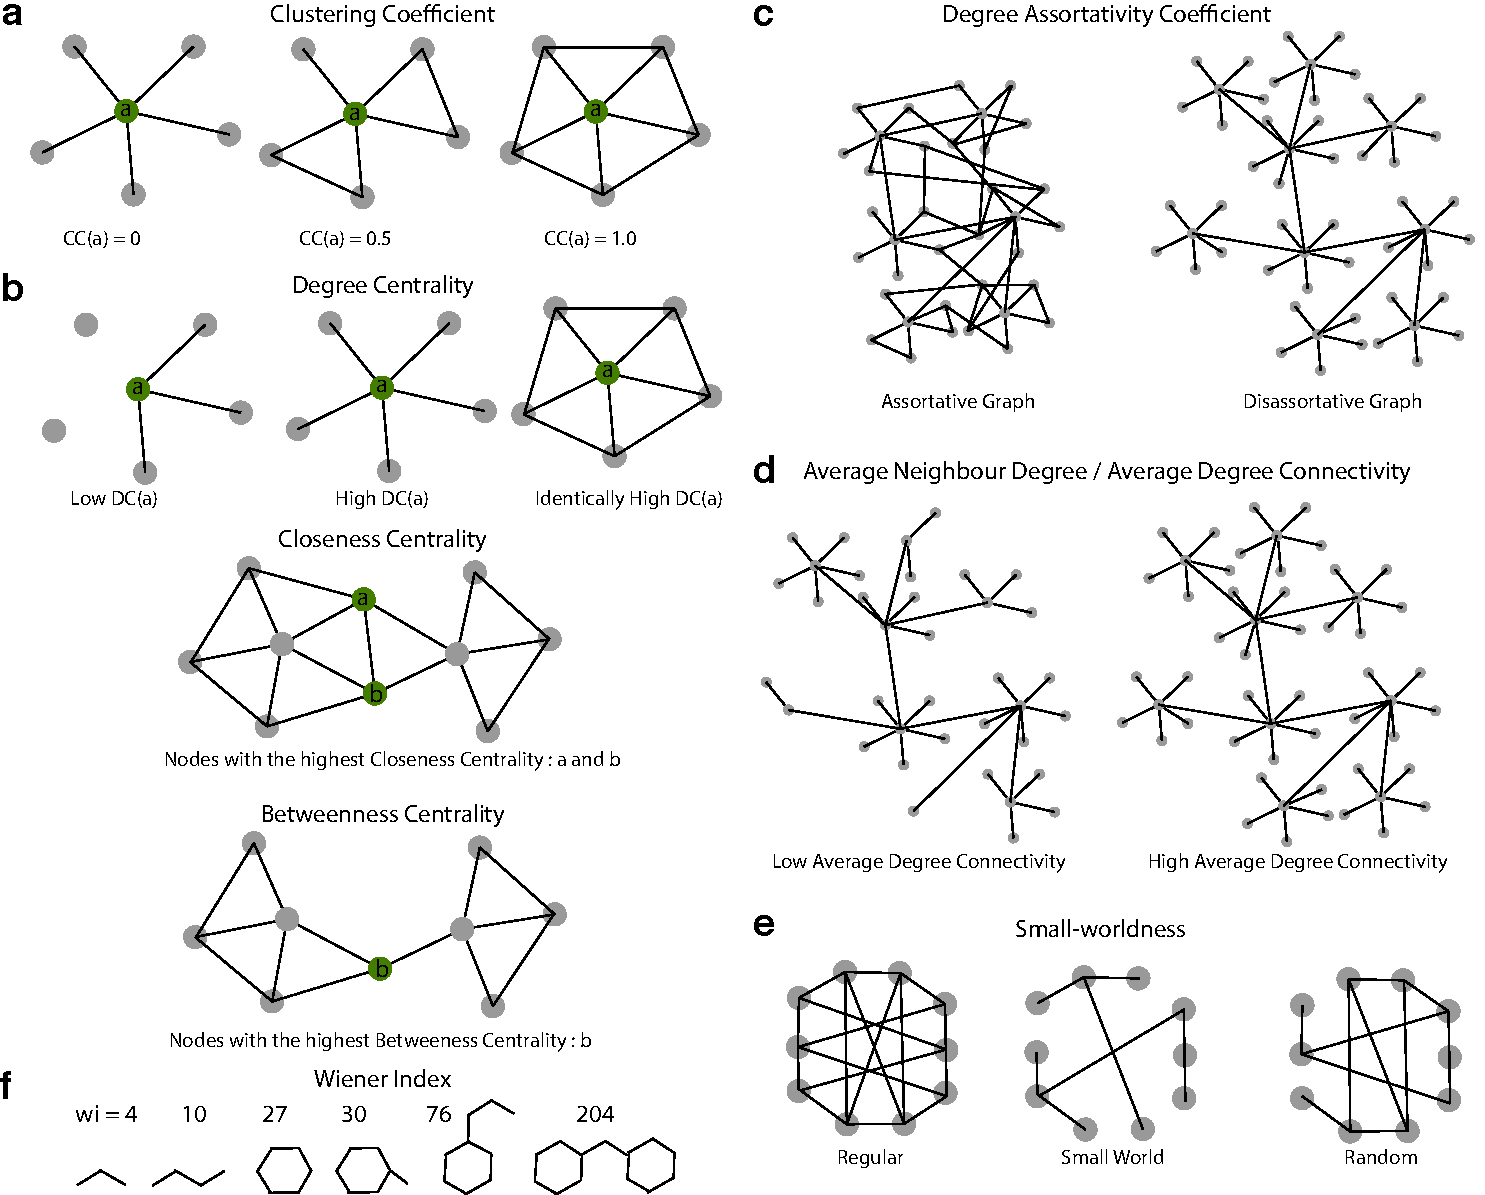
\includegraphics[width=1.\textwidth]{fig/chap5_mnist.pdf}
%\caption[Classification of images with a predictive neural network.]{Classification of images with a predictive neural network. (a) %MNIST with hog below (b) Structure of the neural network. }
%\label{fig_chap5_mnist} 
%\end{figure} 

%Unsurprisingly, the network is able to achieve high accuracy on this classification task. One interesting result, however, is that increased input variance also increases the time to maximum accuracy, and even more so if the learning of inverse variance is disabled (i.e., set to identity matrices). This implies that learning the variance actually helps the neural network perform the classification task. As such, it is interesting to compare these inverse variance matrices, as we did in macaque \gls{V1}, and observe whether differences are taking place.

%\begin{figure}[h!tbp]
%\vspace{0.1cm}
%\centering
%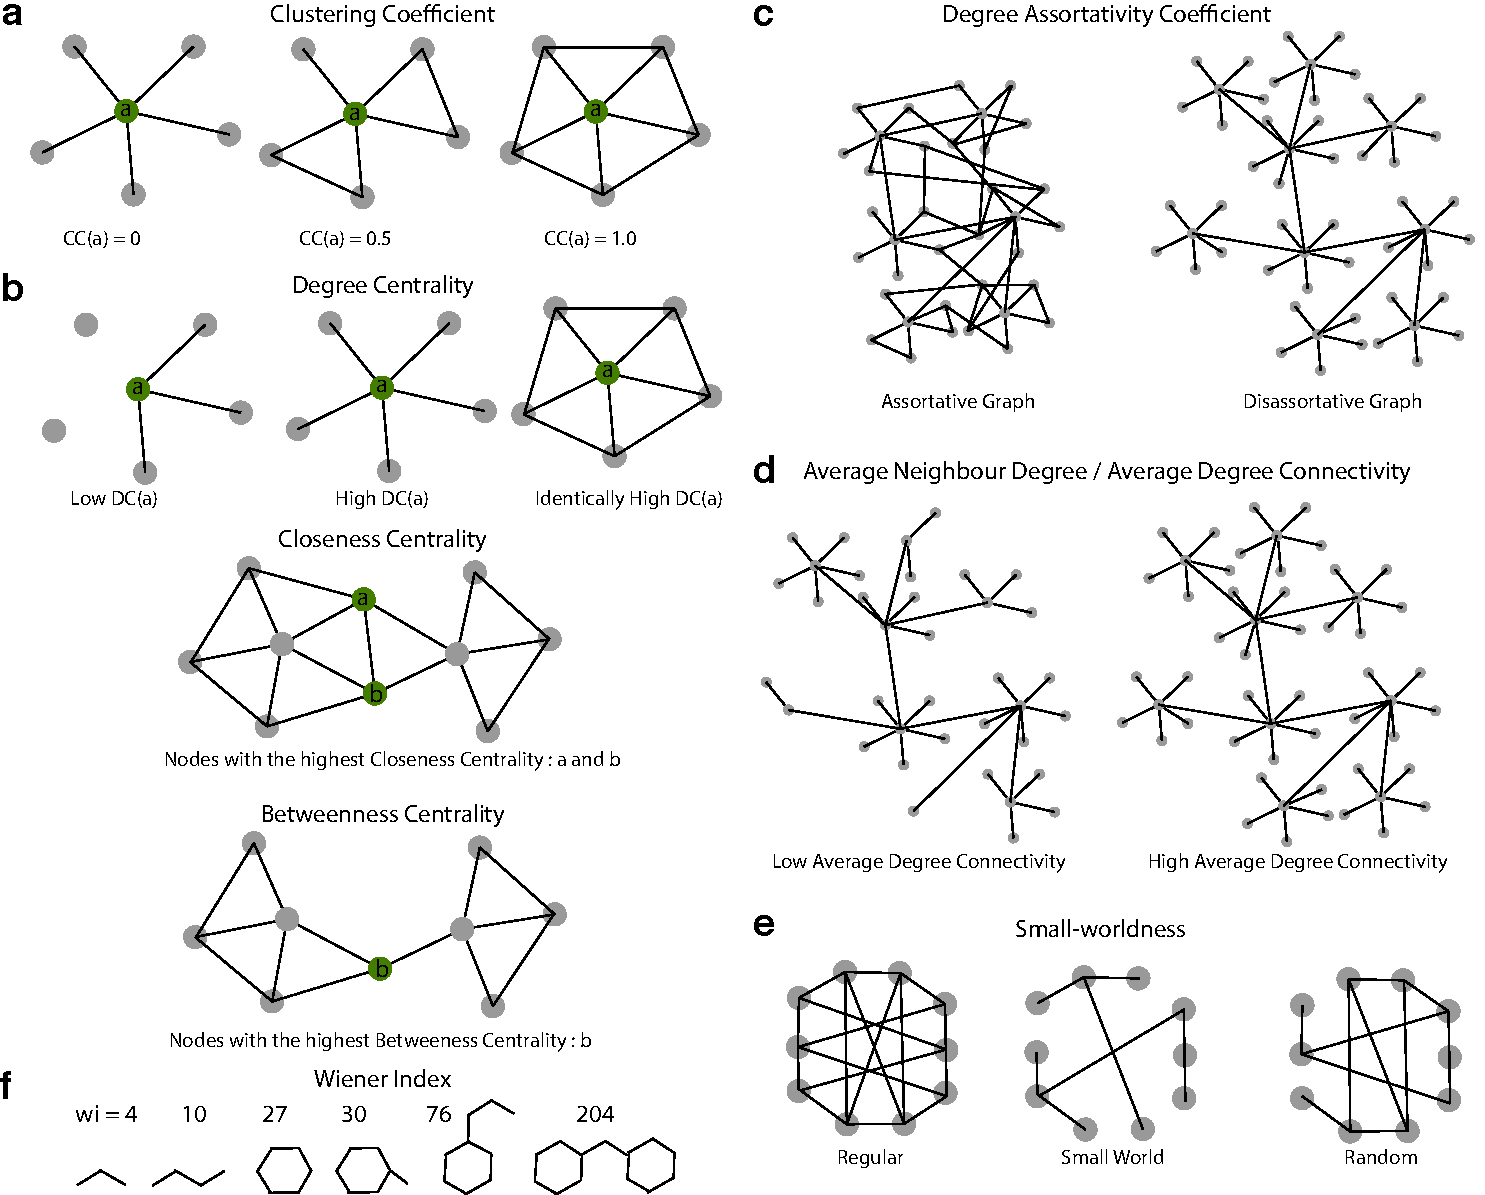
\includegraphics[width=1.\textwidth]{fig/chap5_mnist_matrices.pdf}
%\caption[Inverse variance matrices of a predictive neural network.]{Inverse variance matrices of a predictive neural network. (a) }
%\label{fig_chap5_mnist_matrices} 
%\end{figure} 

% Indeed, as shown in Figure~\ref{fig_chap5_mnist_matrices}, there are striking similarity between these computational matrices and the data extracted from \gls{V1} recordings. Given that the neural network had to explicitely learn the variance of the input, this could indeed suggest that the dynamical restructuring of \gls{V1} are indeed related to learning the sensory variance of the world.